%!TEX root = ../Thesis.tex
\section*{Anhang}
\addcontentsline{toc}{section}{Anhang}
\fancyhead[R]{Anhang}

\anhangsverzeichnis

\anhang{Abbildungen}

\begin{figure}[hbt]
    \centering
    \begin{minipage}[t]{.8\textwidth}
        \caption[]{Auswertung der Daten des S\&P500 im Zeitraum 01-01-1970 bis 24-06-2021 in grafischer Form}
        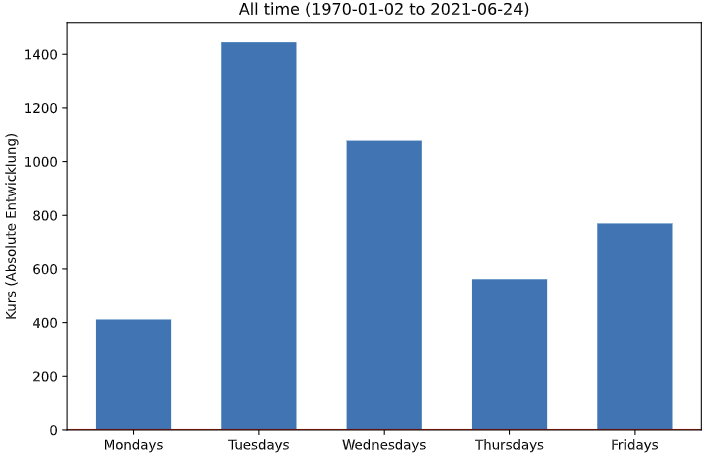
\includegraphics[width=1\textwidth]{img/Auswertung_SP500_1970-2021.PNG}\\
        \source{eigene Darstellung}
        \label{fig:auswertung_sp500_graph}
    \end{minipage}
\end{figure}

\begin{figure}[!htb]
    \centering
    \begin{minipage}[t]{0.8\textwidth}
        \caption{Auswertung S\&P500 - 1980 bis 1990}
        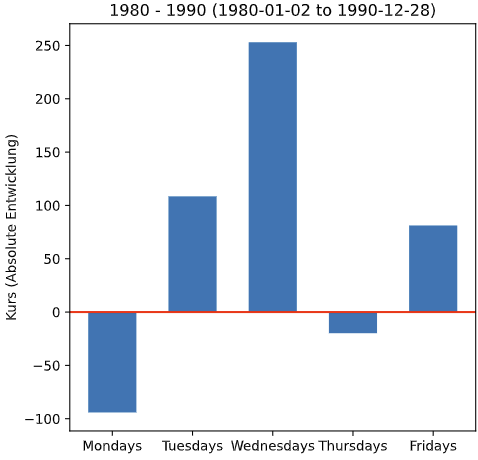
\includegraphics[width=1\textwidth]{img/Auswertung_SP500_1980-1990.PNG}\\
        \source{eigene Darstellung}
        \label{fig:ausw_sp500_1980_1990}
    \end{minipage}
\end{figure}

\clearpage

\anhang{Tabellen}

% \begin{table}[hbt]
%     \centering
%     \begin{minipage}[t]{1\textwidth} % Breite, z.B. 1\textwidth		
%         \caption{User-Stories für Android} % Überschrift
%         \begin{tabularx}{\columnwidth}{ |c|X| }
%             \hline
%             \textbf{Id} & \textbf{Beschreibung}                                                                                                                                                                              \\
%             \hline
%             IT-5373     & Als Verkäufer möchte ich alle Modelle im Sortiment, nach Sparten organisiert, mit Vorschaubildern und Namen betrachten können, um schnell einen Überblick über die verfügbaren Modelle zu bekommen \\
%             \hline
%             IT-5374     & Als Verkäufer möchte ich die Eigenschaften und unterstützten Funktionen zu einem Modell einsehen können, um den Kunden darüber informieren zu können
%             \\
%             \hline
%             IT-5375     & Als Verkäufer möchte ich die Typen eines Modells einsehen können, um mögliche Kombinationen für einen Kunden erstellen zu können                                                                   \\
%             \hline
%             IT-5376     & Als Verkäufer möchte ich Bilder zu einem Modell einsehen können, um damit den Kunden etwas visuelles zeigen zu können                                                                              \\
%             \hline
%             IT-5378     & Als Verkäufer möchte ich ein Modell nach seinem Namen suchen können, um bekannte Modelle schnell zu finden                                                                                         \\
%             \hline
%             IT-5379     & Als Verkäufer möchte ich alle Modelle nach ihren Eigenschaften filtern können, um damit neue Modelle nach Kundenwünschen finden zu können                                                          \\
%             \hline
%             IT-5380     & Als Verkäufer möchte ich alle Modelle einer bestimmten Sparte nach ihren Eigenschaften filtern können, um meine Suche einzugrenzen                                                                 \\
%             \hline
%             IT-5381     & Als Verkäufer möchte ich alle Funktionen und ggf. Videos dazu einsehen können, damit ich die Endkunden über die Funktionsweise und Bedienung informieren kann                                      \\
%             \hline
%             IT-5382     & Als Verkäufer möchte ich alle verfügbaren Bezüge einsehen können, um den Kunden alle Möglichkeiten aufzeigen zu können
%             \\
%             \hline
%             IT-5383     & Als Verkäufer möchte ich alle Farben zu einem Bezug einsehen können, um den Kunden über die Bezugsvarianten informieren zu können                                                                  \\
%             \hline
%             IT-5384     & Als Verkäufer möchte ich über Neuigkeiten (Messen, Schulungen) der Polipol-Gruppe informiert sein, um bei Bedarf an diesen teilzunehmen                                                            \\
%             \hline
%             IT-5385     & Als Verkäufer möchte ich die Webseite der Polipol-Gruppe aufrufen können, um mehr über den Möbelhersteller zu erfahren                                                                             \\
%             \hline
%         \end{tabularx}
%         \source{eigene Darstellung}
%         \label{tab:user_stories}
%     \end{minipage}
% \end{table}

\clearpage